\chapter{Implementation} \label{ch:implementation}

\section{User Interface}
\begin{figure}
	\centering
	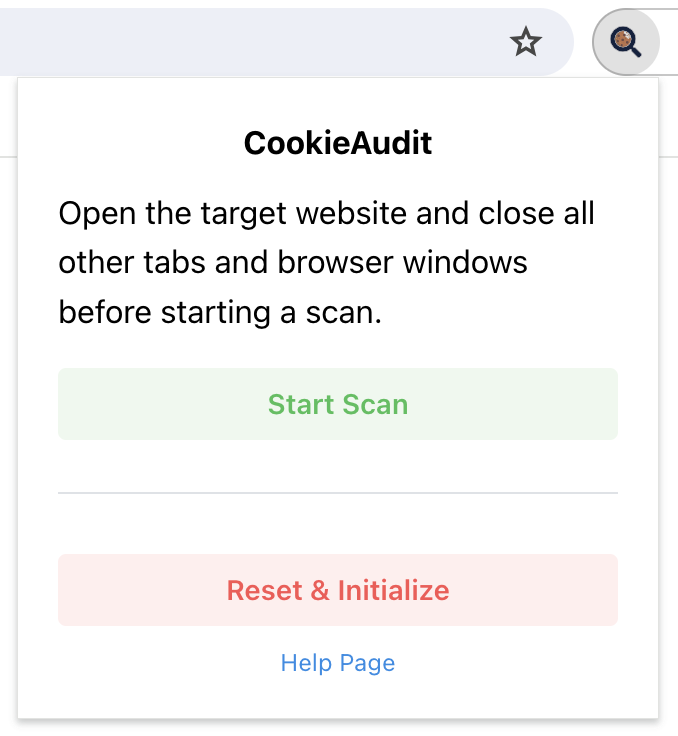
\includegraphics[width=0.5\linewidth]{screenshot_popup.png}
	\caption{Popup window of CookieAudit}
	\label{fig:screenshot-popup}
\end{figure}
The primary way for users to interact with a browser extension is through its popup.
It can be opened by clicking the extension's action icon in the browser toolbar.
Popups are programmed using the same web technologies as websites: HTML, CSS, and JavaScript.
In CookieAudit, users can initiate a website scan, stop it, or download a report summarizing the scan results via the popup.
Additionally, CookieAudit displays real-time information about the scan's progress.
For developing the popup's user interface, we chose to use the React JavaScript library.
React offers a declarative programming model that keeps the displayed data synchronized with the underlying data storage.

\section{Cookie Notice Selection}
CookieAudit is designed to automatically analyze and interact with arbitrary cookie notices. 
However, cookie notices are implemented as standard HTML elements, which makes universal identification challenging.
Next, we present some approaches to find cookie notices in websites.

\subsection{Automatic Selection}
\subsubsection{Crowd-sourced Selectors}
HTML elements can be identified with \emph{selectors}. 
Crowd-sourced efforts, such as EasyList Cookie (\href{https://github.com/easylist/easylist}{github.com/easylist/easylist}), maintain lists of cookie notice selectors.
Automated crawlers by Kampanos et al.~\cite{kampanos2021accept} and Bouhoula et al.~\cite{bouhoula2023automated} have used EasyList to find potential cookie notices on websites.

\subsubsection{Stack Level}
The \emph{z-index} is a CSS property of HTML elements that makes elements with a high index appear above elements with a low index. 
Because a user should quickly see a cookie notice, websites can use a high \emph{z-index} on the notice to let it cover the rest of the website. 
This qualifier has been used by Khandelwal et al.~\cite{khandelwal2023automated} and Bouhoula et al.~\cite{bouhoula2023automated}.

\subsection{User-Aided Selection} \label{subsec:userAidedSelection}
Fortunately, CookieAudit is a browser extension that is used manually.
We can therefore rely on user help by using a cookie notice selector tool.
To specify the element containing a notice, users only needs to hover the mouse over it and then confirm the selection. 
An example can be seen in \cref{fig:screenshot-selection}.

\begin{figure}
	\centering
	\begin{minipage}{0.48\textwidth}
		\centering
		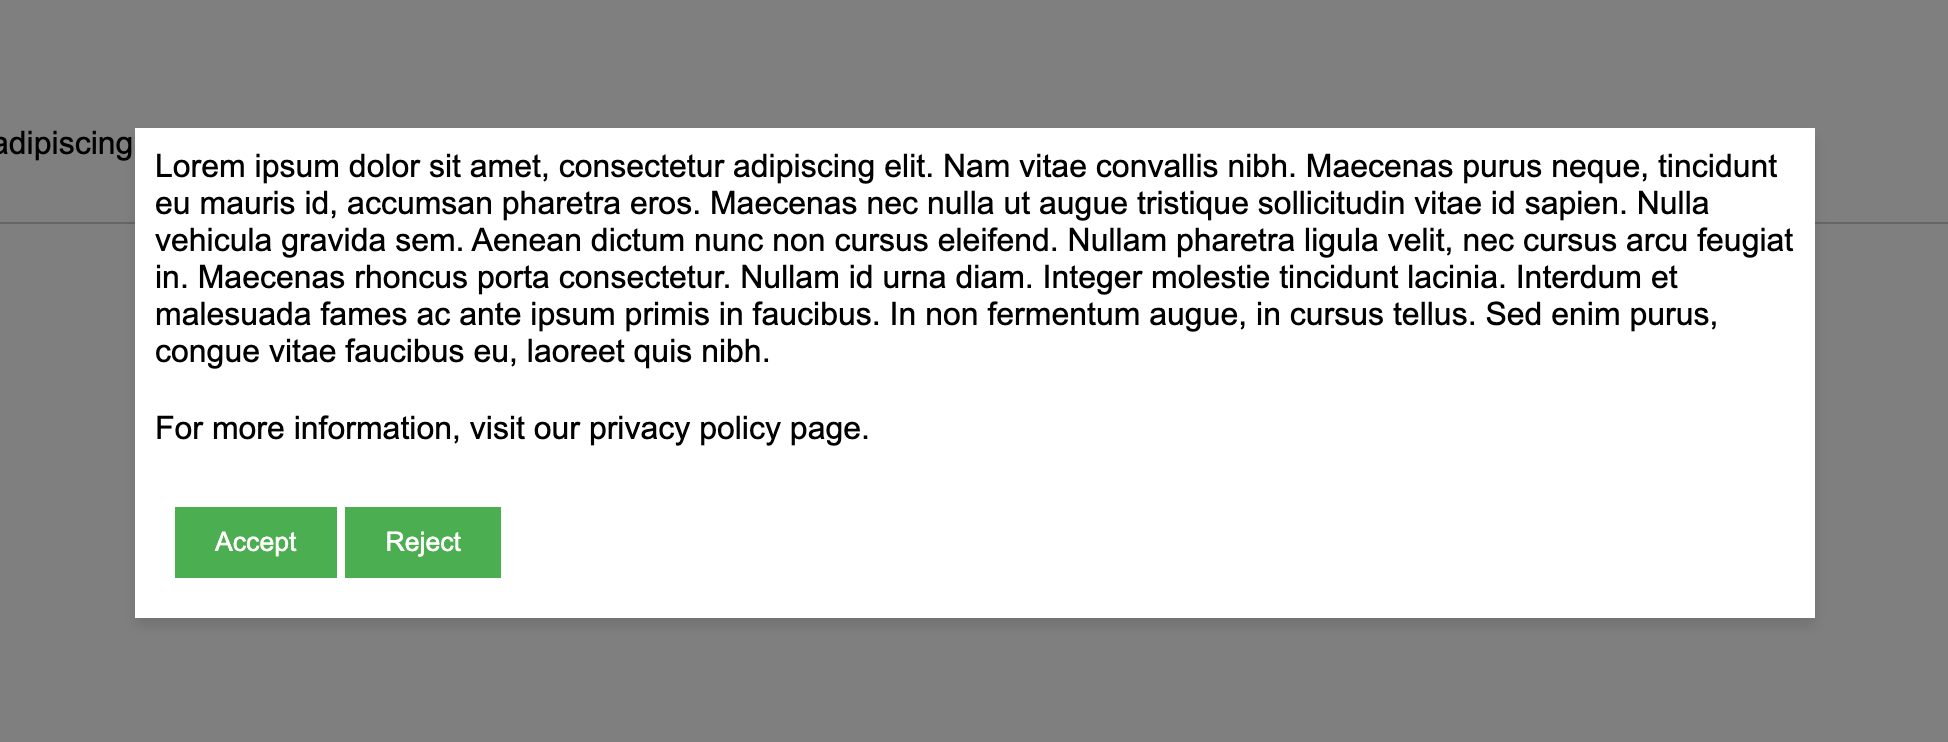
\includegraphics[width=1.0\linewidth]{media/screenshot_unselected.png}
	\end{minipage}\hfill
	\begin{minipage}{0.48\textwidth}
		\centering
		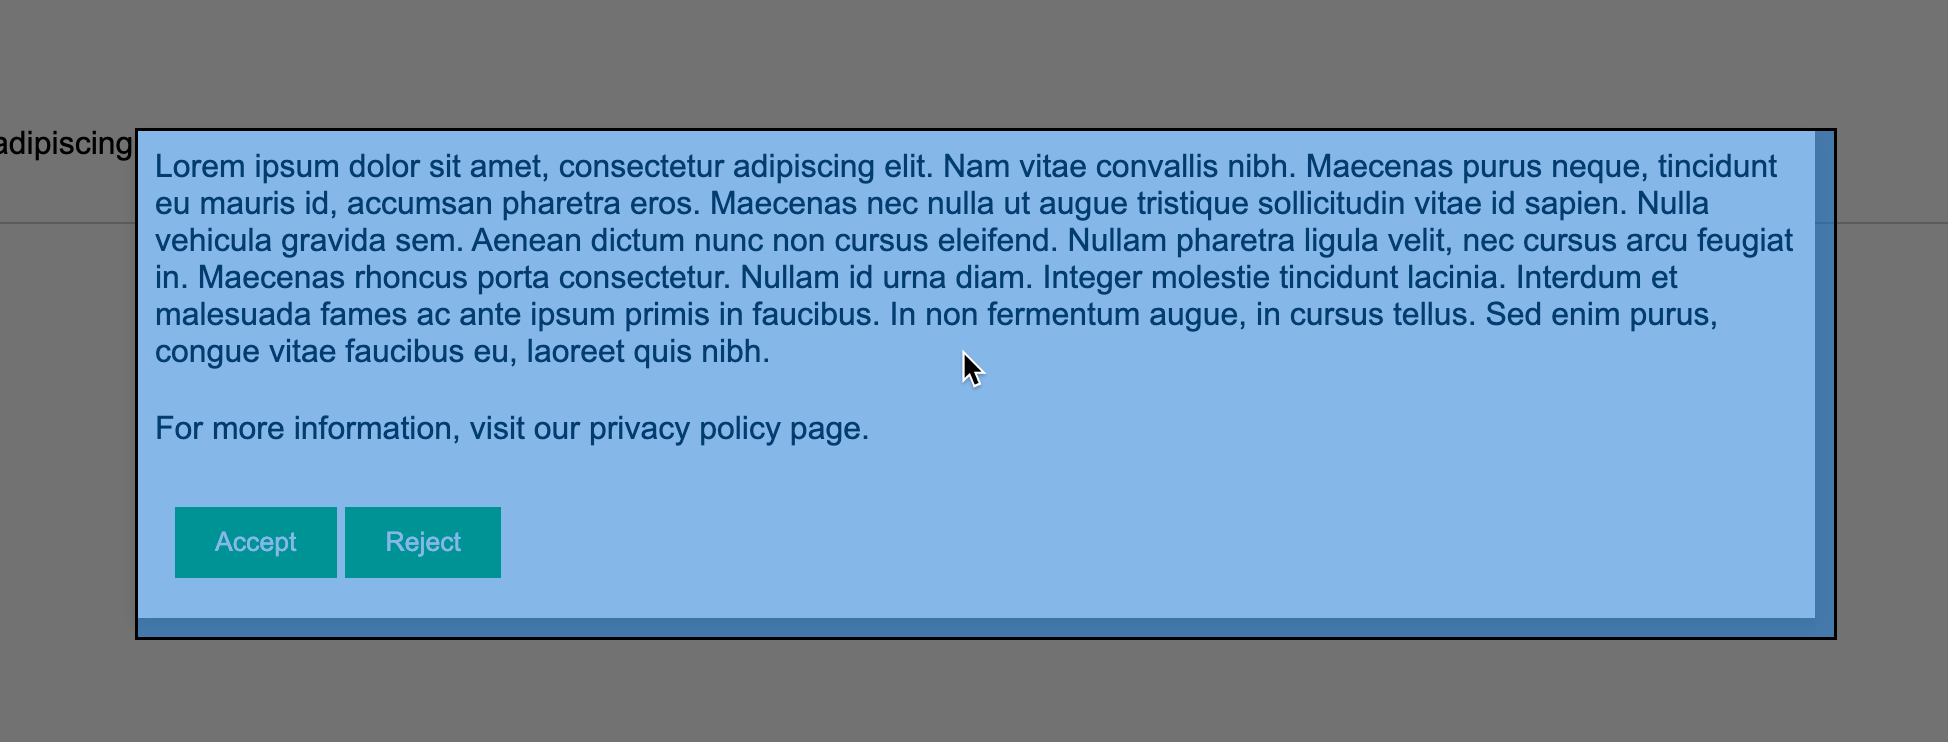
\includegraphics[width=1.0\linewidth]{media/screenshot_selected.png}      
	\end{minipage}
	\caption{Manual notice selection.}
	\label{fig:screenshot-selection}
\end{figure}

The selector is implemented as a \emph{content script}. Content scripts are JavaScript programs which are executed in the context of a web page. 
They can read and change the HTML and CSS of the web page. 
Additionally, they can communicate with the core of the browser extension via messages and by reading and writing to a shared key-value store.

The activated selector listens for cursor movement by the user. 
On movement, it reads the coordinates of the cursor and determines the HTML element at that position.
The selector changes the styling of the determined element to provide users with visual feedback.
By clicking on the highlighted element, users can make an initial selection.
CookieAudit needs users to select the element corresponding to the complete cookie notice. 
Sometimes the desired element is only a container whose area is entirely filled out by the children (see \cref{fig:notice-fillout}).
In this case, every click inside the notice will select a child element rather than the entire notice container. 
Therefore, users won't be able to select the whole notice by simply hovering the cursor.

\begin{figure}
	\centering
	\begin{minipage}{0.48\textwidth}
		\centering
		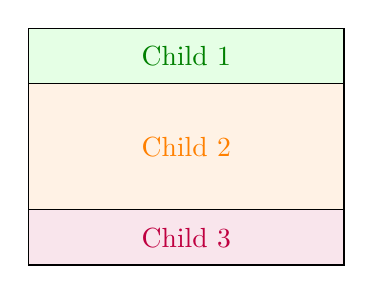
\begin{tikzpicture}[]
			% Outer box
			\draw [thick] (0,0) rectangle (4,-3);
			
			% Child boxes
			\draw [fill=green!10] (0,0) rectangle (4,-0.7) node[midway, text=green!50!black] {Child 1};
			\draw [fill=orange!10] (0,-0.7) rectangle (4,-2.3) node[midway, text=orange] {Child 2};
			\draw [fill=purple!10] (0,-2.3) rectangle (4,-3) node[midway, text=purple] {Child 3};
		\end{tikzpicture}
	\end{minipage}\hfill
	\begin{minipage}{0.48\textwidth}
		\centering
		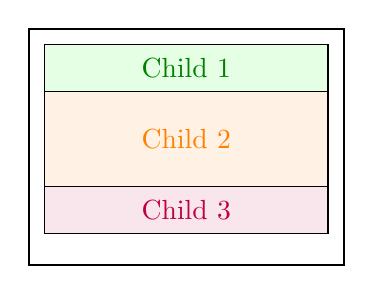
\begin{tikzpicture}[]
			% Outer box
			\draw [thick] (0,0) rectangle (4,-3);
			
			% Child boxes
			\draw [fill=green!10] (0.2,-0.2) rectangle (3.8,-0.8) node[midway, text=green!50!black] {Child 1};
			\draw [fill=orange!10] (0.2,-0.8) rectangle (3.8,-2) node[midway, text=orange] {Child 2};
			\draw [fill=purple!10] (0.2,-2) rectangle (3.8,-2.6) node[midway, text=purple] {Child 3};
		\end{tikzpicture}     
	\end{minipage}
	\caption{Any location in the left notice will map to one of the children. Only the white area in the right notice will be mapped to the whole notice.}
	\label{fig:notice-fillout}
\end{figure}

As a solution we implemented a context menu that appears after the user has clicked on an element.
With the menu, the user can traverse up the tree to the element containing the whole cookie notice.
In the end, the selection can be confirmed with a separate button.

Because of the heterogeneity of the web, we encountered several edge cases resulting from the implementation details of cookie notices. 
Next, we will present our solutions.

\subsubsection{Inline Frame}
An inline frame allows developers to embed another HTML context by linking to a URL~\cite{iframeMdn}.
Some websites implement cookie notices with an \verb|iframe| that refers to a Consent Management Platform.
To enable users to select the cookie notice, we inject the \emph{selector} content script not only into the original web page, but also into all \verb|iframe| elements.

\subsubsection{Shadow DOM}
A shadow DOM separates elements inside of it from the influence of the main document's JavaScript and CSS~\cite{shadowDomMdn}.
Some developers use this feature to integrate cookie notices into their web page.
This encapsulation prevents our selector content script from directly accessing the cookie notice elements. 
To address this, we implement a solution during user notice selection:

As described before, we continuously query for the element that is located at the user's cursor coordinates.
When a user hovers over an element within a shadow DOM, this query will return the root of the shadow DOM (the \emph{shadow root}). 
We then check if the element is indeed a shadow root by reading the \verb|shadowRoot| property of the HTML element.
If so, we explicitly enter the shadow DOM context and query for the element at the user's cursor coordinates. 


\subsubsection{Dialog Element}
The \verb|dialog| element is an HTML element that can be used to build dialog boxes such as cookie notices.
When opened, it displays above all elements of the website and will cover elements with arbitrary \verb|z-index| values. 
Multiple \verb|dialog| elements are stacked based on their opening order, with the most recent dialog displayed on top.
If used to display a cookie notice, a dialog element would also hide our selector context menu.
Therefore, we have implemented the menu with a \verb|dialog| element.
By opening our dialog after the cookie notice renders, we ensure that the menu will be visible and accessible to CookieAudit users.

\section{Cookie Notice Analysis}
As a part of the scan, CookieAudit needs to analyze the text and buttons inside the cookie notice.
CookieAudit automatically checks if the text inside a cookie notice declares the actual cookie usage properly. Secondly, it classifies the buttons by their functionality, e.g., \emph{Open Settings}.

We will use functionality implemented in the automated crawler by Bouhoula et al.~\cite{bouhoula2023automated} to extract and classify the elements of the cookie notice. 

\subsection{Extraction} \label{subsec:extraction}
To extract the cookie notice text, we iterate through all visible elements inside the notice and concatenate their text content.
For nested elements, which are common in HTML's tree-like structure, we recursively repeat this process.

To enable automated interaction with cookie notices, CookieAudit needs to identify all clickable elements.
We will use the the criteria proposed by Bouhoula et al.~\cite{bouhoula2023automated}.
First, we will consider only elements of type \verb|div|, \verb|span|, \verb|a|, \verb|button| or \verb|input| that fulfill one of the following criteria: 
has the accessibility (ARIA) role \verb|button|, 
has the attribute \verb|onclick| or
has a non-negative \verb|tabindex|.
Furthermore we consider elements that, when hovered over, change the mouse to a pointer.
The last criterion was added based on manual testing, as it captured some interactive elements missed by the other rules in rare cases.

\subsection{Classification}
From the extracted data (\cref{subsec:extraction}) we want to learn if the text correctly declares the cookie purpose and the function of the interactive elements. 

We rely on the machine learning models developed by Bouhoula et al.~\cite{bouhoula2023automated} for the classificatoin

\subsection{Exploration}
Cookie notices can offer additional settings.
The settings may contain additional text with a declaration of the cookie purpose, or interactive elements e.g, to reject specific cookie categories or even all non-necessary cookies.
If a \emph{Settings} button is available in a cookie notice, clicking it may change the content of the current notice to display the settings, open a new settings notice or open a separate web page with the settings.
Because of the mentioned text contents and interactive elements, CookieAudit needs to analyze the settings.

Similar to the approach implemented by Bouhoula et al.~\cite{bouhoula2023automated}, CookieAudit clicks on all interactive elements that were classified as \emph{Settings}.
If no interactive elements were classified as \emph{Settings}, CookieAudit alternatively uses three \emph{Other} elements. 
In particular elements that are located on the bottom of the cookie notice (by sorting the \emph{Other} elements by their y-coordinates) are used.
This simple heuristic is based on the observation that the \emph{Settings} button is often located at the bottom.
After the \emph{Settings} have been opened and identified, CookieAudit will again proceed as for the original cookie notice: retrieving and analyzing the text and interactive elements.
CookieAudit adds the elements of type \emph{Reject}, \emph{Close} and \emph{Save Settings} to the \textsc{ieToInteract} array as a sequence of selectors: first the \emph{Settings} element selector, then the second layer element selector. 

Based on the work by Bouhoula et al.~\cite{bouhoula2023automated}, we implemented the detection and handling of the following three scenarios:

\subsubsection{New Cookie Notice}
The cookie notice settings can be displayed inside a new notice that appears e.g., above the original cookie notice. 
CookieAudit detects this situation if one of the following criteria holds:

\begin{itemize} 
    \item a query for the cookie notice with the selector returns \verb|null|
    \item the cookie notice is not visible anymore (e.g., if the notice has or inherits an \verb|opacity| of 0, has or inherits the CSS \verb|visibility| of hidden or collapse, or has an area of 1 pixel or less) 
    \item the notice still exists and is visible, but its text content or the dimensions (height and width) have \emph{not} changed after the interactive element click
    \item the cookie notice is covered by another element. CookieAudit runs \verb|elementFromPoint()| at the coordinates of the cookie notice center. If the returned element is not the notice or contained in the notice, we consider the notice covered.
\end{itemize}

To identify the settings element and start the analysis, CookieAudit activates the \emph{Cookie Notice Selector} (as described in \cref{subsec:userAidedSelection}) and lets the user manually select the settings notice.

\subsubsection{New Web Page}
CookieAudit stores the URL of the web page before the interactive element click and compares it to the URL of the web page after the click.
If it has changed, CookieAudit classifies the outcome as a new notice on a separate web page.

Also in this case CookieAudit starts the \emph{Cookie Notice Selector}. 
The selector can be used to select both settings that are part of the normal flow of the web page, or displayed as a hovering dialog.
After the user selection and subsequent settings analysis, CookieAudit returns to the URL where the scan was started.

\subsubsection{Same Cookie Notice}
If neither the criteria of a \emph{New Cookie Notice} nor \emph{New Web Page} apply, CookieAudit assumes the settings to be now contained in the original cookie notice.
This effectively means that the original cookie notice is still visible, the contents or dimensions have changed and the URL of the web page is still the same.
CookieAudit directly starts the settings notice analysis without any user interaction.

\section{Dark Pattern Detection}
\section{Managing Page Loads and Changes}
\section{Report Creation}